\section{Transportschicht}
\begin{figure}[H]\centering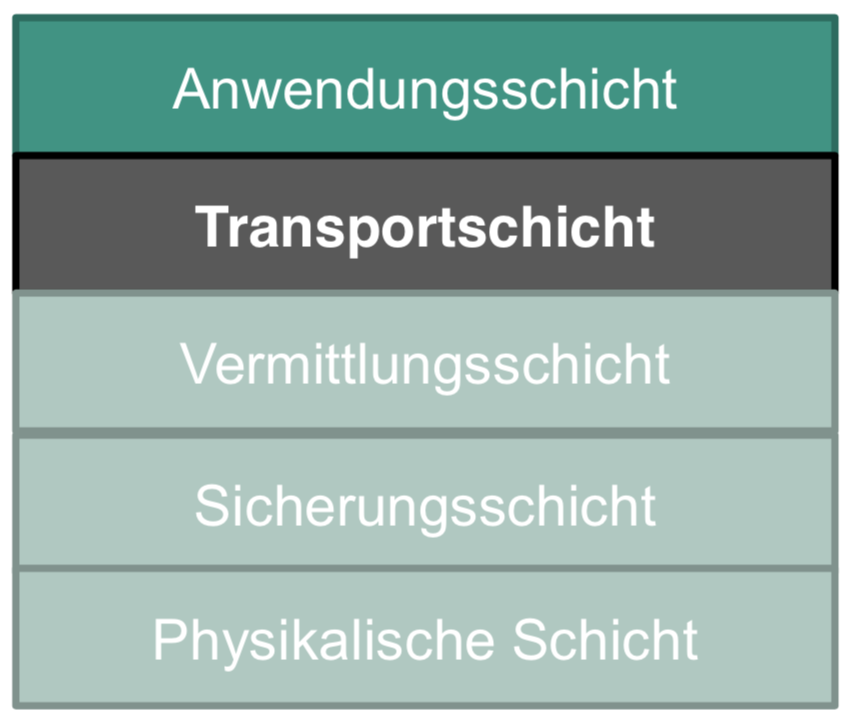
\includegraphics[width=80px]{SchichtTransport}\end{figure}
%\paragraph{Internet-Protokollstack}
%\begin{items}
%  \item Anwendungsschicht
%  \item \textbf{Transportschicht}
%  \item Vermittlungsschicht
%  \item Sicherungsschicht
%  \item Physikalische Schicht
%\end{items}

\paragraph{Ziele und Prinzipien}
\begin{items}
	\item Kommunikation zwischen Prozessen
  \item \emph{Verbergen von Transportdetails vor höheren Schichten}
  \item \emph{Bereitstellung von Transportdiensten} \\*
    \( \leadsto \) logische \textbf{Nutzer-zu-Nutzer-Kommunikation} (Anwendungen)\\*
    Vermittlungsschicht: Ende-zu-Ende-Kommunikation (Endsysteme)
    \medskip
  \item Transportprotokoll läuft auf Endsystemen
  \item \textbf{Sender}: \\*
    - \emph{Segmentieren} von Anwendungsnachrichten \\*
    - \emph{Weiterleiten} an Vermittlungsschicht
  \item \textbf{Empfänger}: \\*
    - \emph{Reassemblieren} der Segmente in Nachrichten \\*
    - \emph{Weiterleiten} an Anwendungsschicht
\end{items}

\paragraph{Protokolle}
\begin{items}
  \item \textbf{UDP} (\emph{user datagram protocol}): \\*
    bietet verbindungslosen, \textbf{unzuverlässigen} Transportdienst
  \item \textbf{TCP} (\emph{transmission control protocol}): \\*
    bietet verbindungsorientierten, \textbf{zuverlässigen} Transportdienst
    \medskip
  \item \textbf{Unzuverlässig}: keine Fehlermaßnahmen\\*
    \( \leadsto \) unklar, wie viel der gesendeten Daten korrekt ankommt
  \item \textbf{Zuverlässig}: Fehlermaßnahmen garantieren\\*
    - \emph{Korrektheit}, \emph{Vollständigkeit}, \emph{Reihenfolge} \\*
    - keine \emph{Duplikate}, keine \emph{Phantom-Pakete}
\end{items}

\paragraph{(De-)Multiplexing --- Ports}
\begin{items}
\item Ausliefern von Segmenten an den korrekten Socket (nutze Transportheader)
  \item Port = \emph{Adresse der Transportschicht} (Kennzeichnung der Prozesse)
  \item Unstrukturierte Nummer (16 Bit), 0 bis 65535
  \item \textbf{Well known ports}: viele Portnummern unter 1024 für häufig benutzte Anwendungen reserviert (Telnet, HTTP, SMTP, FTP, \dots)
  \medskip
  \item Eindeutige Adressierung eines Prozesses: \dq IP-Adresse : Port\dq (z.B. 129.13.41.1:80)
\end{items}

\paragraph{UDP (User Datagram Protocol)}
\begin{items}
  \item \emph{Sehr einfaches Transportprotokoll mit sehr geringem Overhead (8 Byte)}
  \item \textbf{Eigenschaften}: \\*
    - (De-) Multiplexen von Segmenten für Prozesse \\*
    - \emph{Prüfsumme} für Bitfehler \\*
    - \emph{best effort}: keine Zusagen über Auslieferung bei Empfänger \\*
    - \emph{verbindungslos} \\*
    - \emph{keine Verbindungsaufbauphase}: sofortiges Senden \( \leadsto \) keine weitere Verzögerung \\*
    - \emph{kein Verbindungszustand}: keine Verbindungsinformationen im Endsystem \\* \phantom{-} \( \leadsto \) skaliert z.B. für Server besser\\*
    - \emph{Unreguliertes Senden}: kann Daten so schnell senden wie von Anwendung geliefert \\* \phantom{-} und von Netz abgenommen
  \item \textbf{Verwendung}: \textbf{DNS}, Multimedia (VoIP)
\end{items}
\begin{figure}[H]\centering\label{UDPAufbau}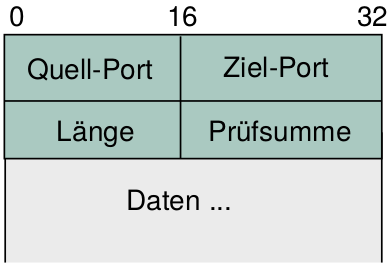
\includegraphics[width=0.2\textwidth]{UDPAufbau}\end{figure}

\pagebreak

\paragraph{Bitfehler}
\begin{items}
  \item \emph{Verfälschung von Bits während dem Datentransport}
  \item \textbf{Ursachen}: Dämpfung, Übersprechen, Synchronisationsverlust, \dots
  \item \textbf{Einzelbitfehler}: ein \emph{einzelnes} Bit fehlerhaft
  \item \textbf{Bündelfehler}: mehrere direkt aufeinanderfolgende Bits fehlerhaft
    \item \textbf{Bitfehlerrate}: Maß für Fehlerhäufigkeit \\*
  \( \text{Bitfehlerrate} = \tfrac{\text{Summe gestörter Bits}}{\text{Summe übertragener Bits}} \)
\end{items}

\paragraph{Bitfehler --- Erkennung/Korrektur}
\newcommand{\dmin}{\ensuremath{d_{\min}}}
\begin{items}
	\item \textbf{Fehlererkennung} (\emph{error detecting code}, EDC)
	\item \textbf{Fehlerkorrektur} (\emph{forward error correction}, FEC)
	\item Hinzufügen von Redundanz (Paritätsbit ($\dmin = 2$), Prüfsumme, \dots)\\*
		\( \leadsto \) Ausreichend stark unterscheidende Codewörter 
	\item \textbf{Hamming-Abstand} $d_{i,j}$: Anzahl Stellen, an denen sich Codewörter unterscheiden
	\item Hamming-Abstand des Codes $\dmin$: Minimaler Abstand zwischen Codewörtern
	\item Erkennen von bis zu $\dmin - 1 $ Bitfehlern
	\item Korregieren von bis zu $\lfloor \frac{\dmin - 1}{2} \rfloor$ Bitfehlern
	\item Kontrollmatrix $H$, für übertragenes Wort $w$ gilt: \\*
		Syndrom $S = w \cdot H^T = 0$, falls Übertragung fehlerfrei ($w$ ist Codewort)\\*
		Ansonsten kann das Syndrom die Position des Bitfehlers angeben
\end{items}

\paragraph{Bitfehler --- Internet-Prüfsumme (UDP, TCP, IP)}
\begin{items}
  \item \textbf{Prinzip}: Aufaddieren aller übertragenen Wörter (16 Bit, als Integer interpretiert), evtl. Übertrag addieren, bitweise negieren (Einerkomplement)
  \item \textbf{Nachteil}: Falsche Reihenfolge kann nicht erkannt werden
\end{items}
\begin{figure}[H]\centering\label{Internetpruefsumme}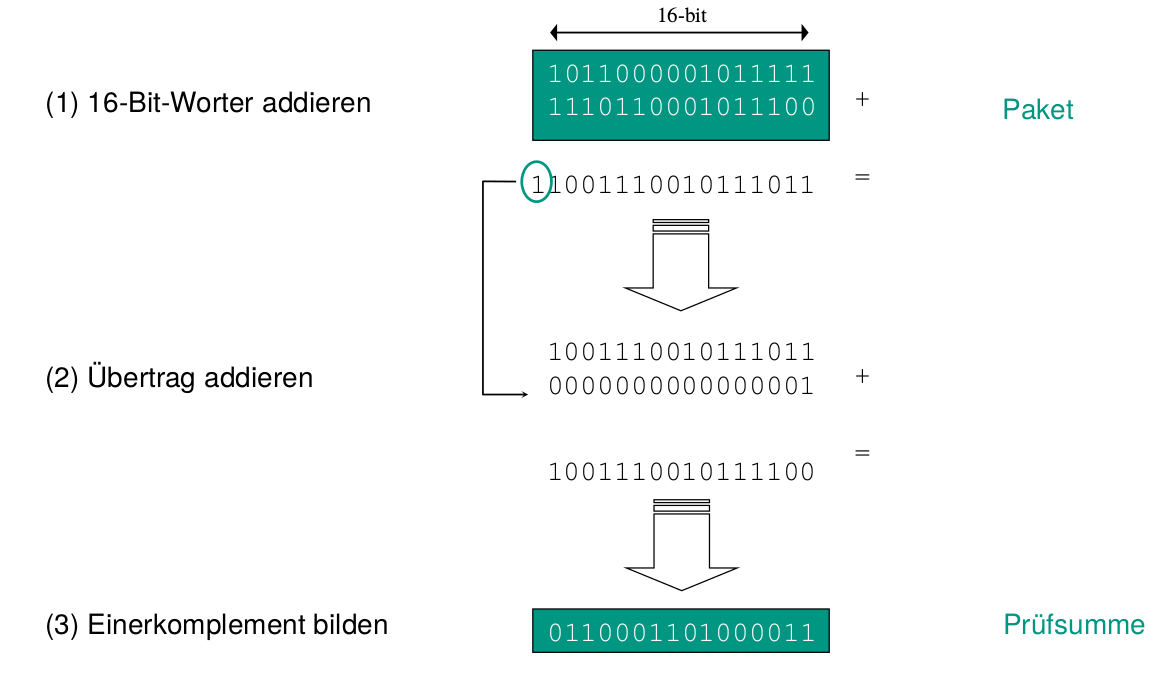
\includegraphics[width=0.33\textwidth]{Internetpruefsumme}\end{figure}

\paragraph{Paketfehler}
\begin{items}
	\item \emph{Verlust / Duplizierung von Paketen}
	\item \emph{Phantom-Pakete}
	\item \emph{Reihenfolgenvertauschung}
	\item \textbf{Ursachen}: \\*
	- Zwischensystemüberlastung \\*
	- Unterschiedliche Wege durch Netz \\*
	- Verfrühte Datenwiederholung, \dots
\end{items}

\paragraph{Paketfehler --- Erkennung/Korrektur}
\begin{items}
  \item \textbf{Sequenznummern} (\emph{sequence number}): \\*
    	- Pakete werden durchnummeriert\\*
    	- Empfänger kann Vollständigkeit, Reihenfolge, Duplikate feststellen
  \item \textbf{Quittungen} (\emph{acknowledgements}) \\*
   - Empfänger informiert Sender, ob Paket angekommen ist \\*
   - \emph{positiv}: Daten erhalten (ACK) / \emph{negativ}: Daten \emph{nicht} erhalten (NACK) \\*
   - \emph{selektiv}: Einzelnes Paket / \emph{kumulativ}: Paketmenge (bis zu einer Sequenznummer)
  \item \textbf{Zeitgeber} (\emph{timer})\\*
    - Sender merkt nicht, wenn ein Paket nicht angekommen ist\\*
    - Nach zeitlicher Obergrenze wird \emph{vermutet}, dass Paket nicht angekommen ist \\* \( \leadsto \) \emph{Sendewiederholung} (\emph{retransmissions})
	\medskip
   \item \textbf{Automatic Repeat Request (ARQ)}\\*
   		Grundlegende Sendewiederholungsvariante:\\*
   		Sender erhält positive Quittungen, kann Sendewiederholungen ausführen
\end{items}

\paragraph{ARQ --- Stop-and-Wait}
\begin{items}
  \item \textbf{Prinzip}: Sender wartet auf Quittung nach jedem gesendeten Paket \\*
    - Erst \emph{nach} Quittungserhalt wird nächstes Paket gesendet \\*
    - Keine Quittung nach Wartezeit (Zeitgeber) \( \leadsto \) Sendewiederholung
  \item \textbf{Sequenznummern}: 1 Bit reicht (Empfänger kann nur Paket doppelt erhalten)
  \item Sehr einfaches ARQ-Verfahren (z.B. im WLAN)
  \medskip
  \item \textbf{Auslastung}: \( U = \tfrac{1}{1+2a} \) (mit \( a = \tfrac{t_a}{t_s} \)) $\qquad (t_{Ges} = t_s + 2t_a)$
  \medskip
  \item $\textbf{a} = \tfrac{t_a}{t_s}$ ist Verhältnis der Länge des Mediums in Bit zur Länge der Dateneinheit
  \item Bandbreitenverzögerungsprodukt \( \tfrac{m}{v}r \)\\*
  Länge des Mediums in Bit\\*
  (Länge \( m \), Ausbreitungsgeschwindigkeit \( v \), Datenrate \( r \))
\end{items}

\paragraph{ARQ --- Go-Back-N}
\begin{items}
  \item \textbf{Zeil}: Leistungsfähigkeit im Vergleich zu Stop-and-Wait erhöhen
  \item \textbf{Prinzip}: Sender sendet mehrere Pakete bis Quittungspflicht \\*
    - Begrenzte Anzahl (\textbf{Fenster}, \emph{window}) an nicht quittierten Paketen \\*
    - Quittierung durch kumulative Quittungen
  \item \textbf{Fehlerfall}: \\*
    - Empfänger empfängt fehlerhaftes Paket, verwirft alle nachfolgenden Pakete\\*
    - Sender wiederholt bei Ablauf des Zeitgebers alle nicht quittierten Pakete
  \item \textbf{Auslastung}: \( U = \begin{cases}
    1 & W \geq 1+2a \\
    \tfrac{W}{1+2a} & \text{sonst}
  \end{cases} \)
\end{items}

\paragraph{ARQ --- Selective Repeat}
\begin{items}
  \item \textbf{Ziel}: Datenaufkommen von Go-Back-N reduzieren
  \item \textbf{Prinzip}: Wie Go-Back-N, Empfänger quittiert selektiv
  \item \textbf{Fehlerfall}: Empfänger puffert und bestätigt nachfolgende, korrekte Pakete \\*
    - Sender wiederholt nur nicht korrekt empfangene Pakete
   \medskip
  \item \textbf{Selective Repeat}: Fehlerhaftes Paket wird nicht bestätigt, Sender wartet auf Timeout
  \item \textbf{Selective Reject}: Empfänger versendet für fehlerhaftes Paket negative Quittung \\*
    - Sender wiederholt sofort und wartet nicht auf Timeout
\end{items}

\paragraph{Paketfehler --- Vorwärtsfehlerkorrektur}
\begin{items}
  \item \textbf{Ziel}: Empfänger muss nur drei von vier Paketen korrekt empfangen um fehlendes Paket rekonstruieren zu können
  \item \textbf{Prinzip}: XOR-Verknüpfung der drei Pakete \( \leadsto \) fehlendes Paket
\end{items}

\paragraph{Flusskontrolle}
\begin{items}
  \item \textbf{Problem}: \emph{Überlastung} von Empfänger durch Sender \( \leadsto \) Datenverlust
   \item Sender muss Größe des Empfangspuffers berücksichtigen
  \item \textbf{Anforderungen}: einfach, fair, stabil, möglichst wenig Netzressourcen nutzen
\end{items}

\paragraph{Flusskontrolle --- Halt-und-Weiter}
\begin{items}
  \item \textbf{Prinzip}: Empfänger sendet \code{halt} und \code{weiter}-Signal
  \item \textbf{Bewertung}: \\*
    - nur auf Vollduplex verwendbar \\*
    - nicht effektiv bei hohen Verzögerungen \\*
    - Probleme bei Verlust der \code{halt}-Meldung
  \item \textbf{Beispiel}: Fast-/Gigabit-Ethernet
\end{items}

\paragraph{Flusskontrolle --- Stop-and-Wait}
\begin{items}
  \item \textbf{Prinzip}: Empfänger sendet Quittung erst, wenn er wieder empfangen kann
   \item Sender wird durch Zurückhalten gebremst
  \item \textbf{Problem}: Sender kann nicht zwischen Datenverlust und Überlastung unterscheiden
\end{items}

\paragraph{Flusskontrolle --- Kreditbasiert}
\begin{items}
  \item \textbf{Prinzip}: \\*
    - Sender kann höchstens \( n \) Pakete unquittiert senden \\*
    - \( n \) = Pufferkapazität des Senders \( \Rightarrow \) \textbf{Sendekredit} \\*
    - Alternativbezeichnung: Fenster (\emph{sliding window}) \\*
    - Fenster wird durch korrekte positive Quittung weitergeschaltet \\*
    - Empfänger kann Kredit bestimmen (z.B. in TCP)
\end{items}

\paragraph{TCP --- Prinzip}
\begin{items}
	\item \textbf{Zuverlässiger}, verbindungsorientierter Transportdienst zwischen Anwendungen
  \item \emph{Erhält Bytestrom von Anwendung (über Socket), übergibt TCP-Segmente an IP}
  \item Wann wird ein TCP-Segment erzeugt und versendet?\\*
    - MSS (\emph{maximum segment size}): Anwendungsdatenlänge (z.B. 1460 Byte) \\*
    - Push (\code{PSH} in TCP-Segmentkopf): Sender verlangt sofortiges Versenden der Daten \\*
    - Zeitgeber: Nach Zeitintervall der Inaktivität vorhandene Daten senden
  \item \textbf{Fehlerkontrolle}: Sequenznr., Prüfsumme, Quittierungen, Sendewiederholungen
  \item \textbf{Sequenznummern}: pro Byte, nicht pro Segment (erstes Byte in Segment, initiale Sequenznummer von Endsystem \emph{zufällig} gewählt)
  \item \textbf{Quittungen: } positive kumulative Quittungen (Sequenznummer des \emph{nächsten} Bytes, das erwartet wird), mit Datensegment versendet (\emph{piggybacked} im Header)
\end{items}
\begin{figure}[H]\centering\label{TCPAufbau}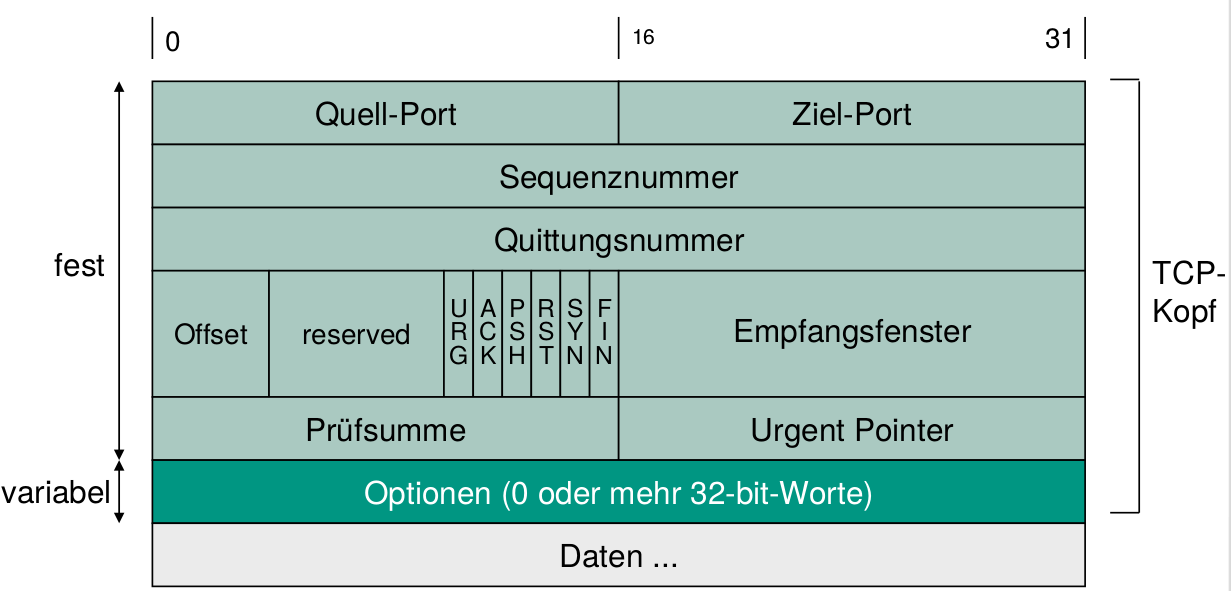
\includegraphics[width=0.33\textwidth]{TCPAufbau}\end{figure}

\paragraph{TCP --- Felder}
\begin{items}
  \item \textbf{Quell-/Ziel-Port}: Identifizieren Verbindungsendpunkte
  \item \textbf{Sequenznummer}: gemessen in Byte, nicht pro Segment
  \item \textbf{Quittung}: nächste von Empfänger erwartete Sequenznummer
  \item \textbf{Offset}: Anzahl 32 Bit-Wörter in TCP-Kopf
  \item \textbf{URG}: 1, falls \emph{urgent pointer} verwendet wird (idR leer)
  \item \textbf{SYN}: Bei Verbindungsaufbau \emph{connection request} oder \emph{connection confirmation}
  \item \textbf{ACK}: Gültigkeit des Quittungsfeldes; unterscheidet bei gesetztem SYN-Bit zwischen Request und Confirmation; 
  \item \textbf{FIN}: Sender möchte nichts mehr senden
  \item \textbf{RST}: Verbindung zurücksetzen
  \item \textbf{PSH}: übergebene Daten sollen sofort weitergeleitet werden (idR leer)
  \item \textbf{Empfangsfenster}: Flusskontrolle
  \item \textbf{Prüfsumme}: Prüfsumme über TCP-Kopf, Daten und Pseudoheader
  \item \textbf{Urgent-Zeiger}: relativer Zeiger auf wichtige Daten
  \item \textbf{Optionen-Feld}: Optionen variabler Länge ($n * 32$ Bit)
\end{items}

\paragraph{TCP --- Flusskontrolle}
\begin{items}
  \item \textbf{Ziel}: Empfänger nicht überlasten
  \item \textbf{Prinzip}: \\*
    - \emph{Empfänger}: reserviert Pufferplatz pro Verbindung (explizite Kreditvergabe) \\*
    \phantom{-} \( \cdot \) \code{RcvBuffer}: gesamter Pufferplatz (default 4096 Byte) \\*
    \phantom{-} \( \cdot \) \code{RcvWindow}: freier Pufferplatz (Empfangsfenster) in TCP-Header mitsenden \\*
    \phantom{-} \( \cdot \) Sender sendet nicht mehr unbestätigt als in \code{RcvWindow} passt
\end{items}
\begin{figure}[H]\centering\label{TCPBuffer}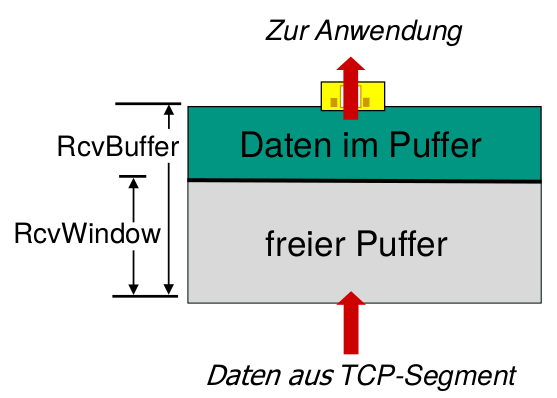
\includegraphics[width=0.2\textwidth]{TCPBuffer}\end{figure}

\paragraph{TCP --- Verbindungen}
\begin{items}
  \item \textbf{Verbindungslos (UDP)}: Daten werden ohne vorherigen Handshake gesendet \\*
    - \emph{Vorteil}: schnelle Datenversendung möglich \\*
    - \emph{Nachteil}: kein Feedback, keine Bestätigung
  \item \textbf{Verbindungsorientiert (TCP)}: Expliziter Verbindungsaufbau/-abbau \\*
    - \emph{Vorteil}: Kommunikationsparameter können ausgehandelt werden \\*
    - \emph{Nachteile}: Verzögerter Datenaustausch, Overhead ggf größer als Daten
    \item Probleme mit 2-Wege-Handshake: Verzögerungen + Wiederholte Nachrichten können zu halboffenen Verbindungen führen
    \item \textbf{3-Wege-Handshake}: SYN, SYN/ACK, ACK (letztes ACK kann Nutzdaten enthalten)
    \item \textbf{Abbau}: Richtungen unabhängig jeweils durch FIN, ACK schließen, danach Warten vor vollständigem löschen (falls Wiederholungen auftreten)
    \item Abbruch: RST, Verbindung wird unmittelbar geschlossen
\end{items}

%\paragraph{TCP --- Zusammenspiel mit HTTP}
%\begin{figure}[H]\centering\label{TCPHTTP}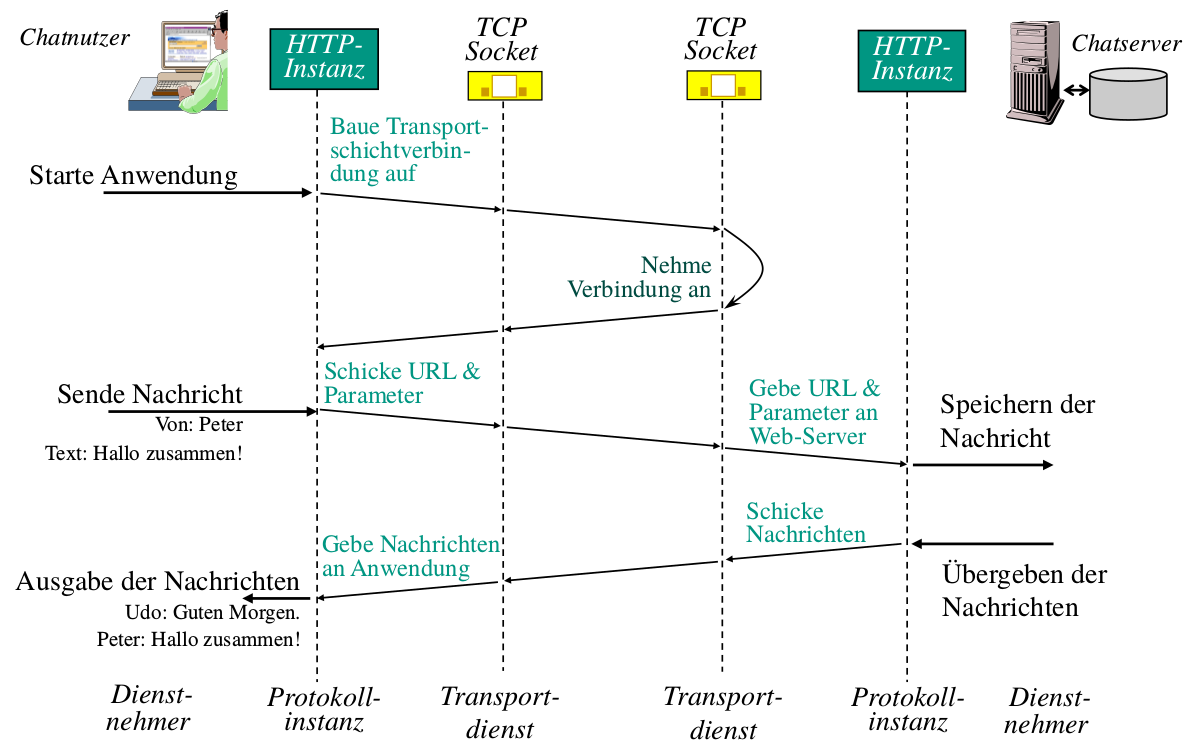
\includegraphics[width=0.4\textwidth]{TCPHTTP}\end{figure}

\paragraph{TCP --- Staukontrolle}
\begin{items}
	  \item \textbf{Ziel}: Netz nicht überlasten (Pufferüberläufe in Routern vermeiden)
	\item \textbf{Staukontrollfenster} (\emph{congestion window}, \code{CWnd}) beschränkt maximale Datenmenge: \\*  \( \text{LastByteSent} - \text{LastByteAcked} \leq \text{min} \{ \text{CWnd}, \text{RcvWindow} \} \)
	\item \textbf{Stauerkennung}: Vermutung einer Stausituation bei ausbleibender Quittung
	\item \textbf{Staubehebung}: Reduktion von \code{CWnd}
	\item Langsames Erhöhen von \code{CWnd} \( \leadsto \) herantasten an Netzkapazität
	\medskip
  \item \textbf{Start}: \code{CWnd} = 1 \code{MSS} (\emph{maximum segment size})
  \item \textbf{Slow-Start}, falls \code{CWnd} \( \leq \) \code{SSTresh} \& Quittungen rechtzeitig da \\*
    - \emph{Exponentielles} Erhöhen \code{CWnd} (\code{CWnd} += 1 bei jeder empfangenen Quittung)
  \item \textbf{Congestion Avoidance}, falls \code{CWnd} > \code{SSTresh} \& Quittungen rechtzeitig da \\*
    - \emph{Lineares} Erhöhen \code{CWnd} (\code{CWnd} += \( \tfrac{1}{\text{\code{CWnd}}} \) bei jeder empfangenen Quittung)
  \item \textbf{Congestion}, falls Quittung nicht rechtzeitig da: Stau vermutet \\*
    - \( \text{\code{SSTresh}} = \text{max}(\tfrac{\text{FlightSize}}{2}, 2*\text{MSS}) \) (FlightSize = unquittierte, gesendete Daten) \\*
    - \code{CWnd} zurücksetzen (neue Slow-Start-Phase): \code{CWnd} = 1 \code{MSS}
\end{items}
\begin{figure}[H]\centering\label{TCPStaukontrolle}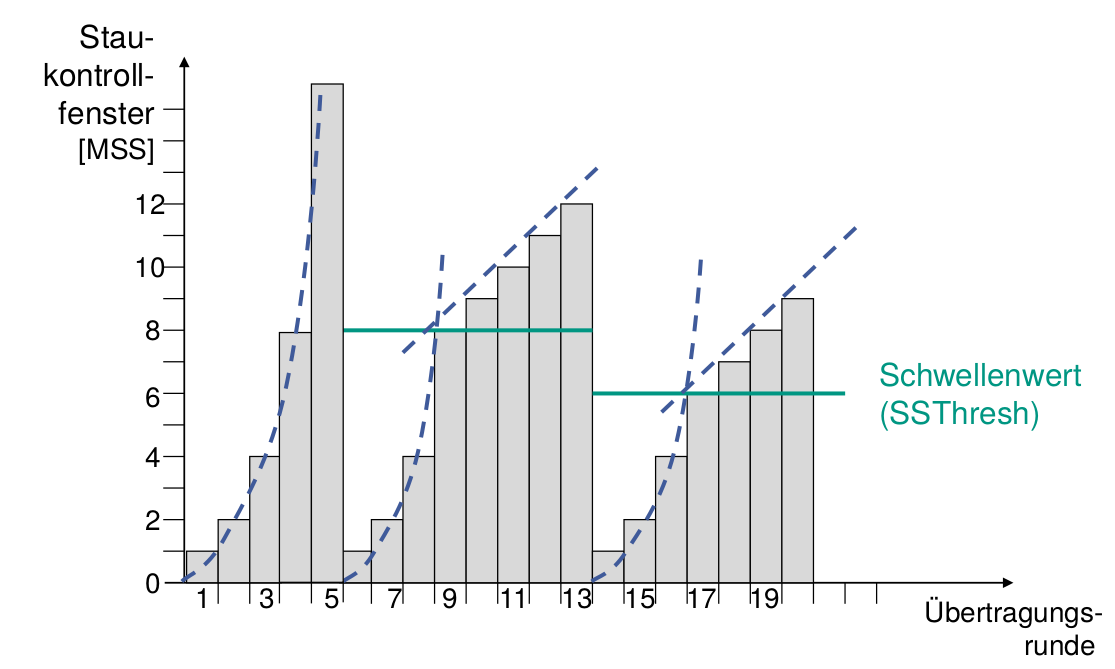
\includegraphics[width=0.33\textwidth]{TCPStaukontrolle}\end{figure}